\documentclass[a4paper,fontset=none]{ctexart}
\usepackage[inner=2.0cm,outer=2.0cm,top=2.5cm,bottom=2.5cm]{geometry}
\usepackage{setspace}
\usepackage[rgb]{xcolor}
\usepackage{subcaption}
\usepackage{amsmath,amssymb,mathrsfs}
\usepackage{fancyhdr}
\usepackage{rotating}
\usepackage{booktabs}
\usepackage{indentfirst}
\setlength{\parindent}{2em}
\setCJKmainfont{SimSun}[BoldFont=Noto Serif CJK SC Bold, ItalicFont=SimSun]
\setCJKsansfont{Noto Sans CJK SC}[RawFeature=+fwid]
\setCJKmonofont{Noto Sans Mono CJK SC}[RawFeature=+fwid]
\newCJKfontfamily\songti{SimSun}[BoldFont=Noto Serif CJK SC Bold]
\newCJKfontfamily\heiti{Noto Sans CJK SC}[RawFeature=+fwid]
\newCJKfontfamily\kaishu{楷体}
\newCJKfontfamily\fangsong{仿宋}
\newCJKfontfamily\lishu{方正隶书简体}
\newCJKfontfamily\yahei{Noto Sans CJK SC}[RawFeature=+fwid]
\newCJKfontfamily\youyuan{方正兰亭圆简体}

\newcommand{\homework}[6]{
    \pagestyle{myheadings}
    \thispagestyle{plain}
    \newpage
    \setcounter{page}{1}
    \noindent
    \begin{center}
        \framebox{
            \vbox{\vspace{2mm}
                \hbox to 6.28in { {\bf 模板标题 \hfill {\small (#2)}} }
                \vspace{6mm}
                \hbox to 6.28in { {\Large \hfill #1  \hfill} }
                \vspace{6mm}
                \hbox to 6.28in { {\it Instructor: {\rm 老师姓名 #3} \hfill Name: {\rm #5}, ID: {\rm #6}} }
                \vspace{2mm}}
        }
    \end{center}
    \markboth{#5 -- #1}{#5 -- #1}
    \vspace*{4mm}
}

\newcommand{\problem}[2]{\fbox{\textbf{Problem #1}}\hfill (#2 points)\bigskip}
\newcommand{\subproblem}[1]{~\newline\textbf{(#1)}}

\usepackage{fontspec,anyfontsize}
\setmonofont{JetBrains Mono NL}
\usepackage{listings}
\usepackage{verbatim}
\lstset{
    language=Python,
    basicstyle=\ttfamily\small,
    aboveskip={1.0\baselineskip},
    belowskip={1.0\baselineskip},
    columns=fixed,
    extendedchars=true,
    breaklines=true,
    tabsize=4,
    prebreak=\raisebox{0ex}[0ex][0ex]{\ensuremath{\hookleftarrow}},
    frame=lines,
    showtabs=false,
    showspaces=false,
    showstringspaces=false,
    keywordstyle=\color[RGB]{144,0,144},
    commentstyle=\color[RGB]{221,0,0},
    stringstyle=\color[RGB]{0,128,0},
    numbers=left,
    numberstyle=\small,
    stepnumber=1,
    numbersep=12pt,
    captionpos=t,
    escapeinside={\%*}{*)}
}

\begin{document}
\homework{ 模板标题 }{Due: 模板日期 }{}{}{学生姓名}{学号}

\problem{1: Template Problem 1}{10+10+10+20=50}

\begin{table}[ht]
\centering
\begin{tabular}{@{}lll|l@{}}
    \toprule
    \textit{Weather} & \textit{Food} & \textit{Meeting} & \textit{Attend?} \\ \midrule
    cold             & full          & yes              & yes              \\
    cold             & empty         & no               & no               \\
    hot              & full          & yes              & yes              \\
    cold             & full          & no               & yes              \\
    hot              & empty         & no               & no               \\ \bottomrule
\end{tabular}
\caption{Dataset A\label{table:1}}
\end{table}


\subproblem{a} Bessel Function
\[
J_{\nu}(x)=\sum_{k=0}^{\infty}\dfrac{(-1)^k}{k!\Gamma(k+\nu+1)}\left(\dfrac{x}{2}\right)^{2k+\nu}
\]

\subproblem{b}
\begin{lstlisting}
    import numpy as np
    import matplotlib.pyplot as plt
    from matplotlib import cm
    import math
    from matplotlib.pylab import mpl
    from mpl_toolkits.mplot3d import Axes3D

    u = np.linspace(-3 , 3 , 101)
    x , y = np.meshgrid(u , u)
    print("x = \n" , x)
    print("y = \n" , y)

    z = np.exp(-(x**2 + y**2) / 2) / math.sqrt(2 * math.pi)

    fig = plt.figure()
    ax = fig.add_subplot(111, projection = '3d')
    ax.plot_surface(x , y , z, rstride = 2, cstride = 2 , cmap = cm.get_cmap('winter'), linewidth = 0.5)
    plt.show()
\end{lstlisting}

\begin{figure}[ht]
\centering
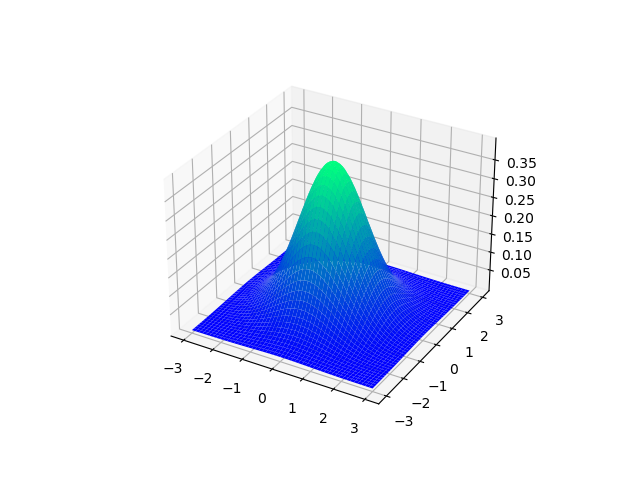
\includegraphics[width=0.8\linewidth]{Template_Picture.png}
\end{figure}

\subproblem{d}
\begin{center}
赴戍登程口占示家人二首（其二）
\medskip

\fangsong{【清】林则徐}
\bigskip

\kaishu{
    力微任重久神疲，再竭衰庸定不支。

    苟利国家生死以，岂因祸福避趋之！

    谪居正是君恩厚，养拙刚于戍卒宜。

    戏与山妻谈故事，试吟断送老头皮。
}
\end{center}

\newpage
\problem{2: Template Problem 2}{5+5+10=20}

\subproblem{a}
\includegraphics[width=0.5\textwidth]{example-image-a}

\subproblem{b}
\includegraphics[width=0.5\textwidth]{example-image-b}

\subproblem{c}
\includegraphics[width=0.5\textwidth]{example-image-c}

\newpage
\problem{3: Template Problem 3}{15+15=30}

\subproblem{a}
可以看到，运行\texttt{list}的\texttt{del}操作符时，数据点集中分布在$t_i=k_{i}n$附近，说明删除第一个或中间某个元素的时间复杂度为O(n)，在本次实验中，$t_1:t_2:t_3:t_4 \approx 4:3:2:1$，与删除点在列表中的位置对应，而删除最后一个元素时，数据点集中分布在水平线$t_5=0.004\,\mathrm{ms}$附近，拟合出的斜率$k_5$几乎为0，说明删除最后一个元素的时间复杂度为O(1)。\\
\indent 推测：这是因为删除列表的第$i$个元素时，需要将后面$n-i$个元素向前移动一位，更改元素指标的时间占大多数。导致删除第一个或中间某个元素的时间复杂度为O(n)，而删除最后一个元素不需要移动其它元素的指标，故时间复杂度为O(1)。

\subproblem{b}
\begin{align*}
    [q,p]_{Q,P}
    &= \frac{\partial q}{\partial Q}\cdot\frac{\partial p}{\partial P} - \frac{\partial q}{\partial P}\cdot\frac{\partial p}{\partial Q} \\
    &= \left(-\frac{\sqrt{1-P^2\mathrm{e}^{2Q}}}{\mathrm{e}^Q} - \frac{P^2\mathrm{e}^Q}{\sqrt{1-P^2\mathrm{e}^{2Q}}}\right)\cdot\left(\frac{-\mathrm{e}^Q}{\sqrt{1-P^2\mathrm{e}^{2Q}}}\right) - \\
    &\quad\left(\frac{-P\mathrm{e}^Q}{\sqrt{1-P^2\mathrm{e}^{2Q}}}\right)\cdot\left(\frac{-P\mathrm{e}^Q}{\sqrt{1-P^2\mathrm{e}^{2Q}}}\right) \\
    &= 1 + \frac{P^2\mathrm{e}^{2Q}}{1-P^2\mathrm{e}^{2Q}} - \frac{P^2\mathrm{e}^{2Q}}{1-P^2\mathrm{e}^{2Q}} \\
    &= 1
\end{align*}

\end{document}